\documentclass{article}
\usepackage[utf8]{inputenc}

\title{Exam 1 Written}
\author{Benny Chen}
\date{\today}

\usepackage{color}
\usepackage{amsthm}
\usepackage{amssymb} 
\usepackage{amsmath}
\usepackage{listings}
\usepackage{xcolor}
\usepackage{listings}
\usepackage{graphicx}
\usepackage{enumitem}
\usepackage{pdfpages}
\usepackage[hidelinks]{hyperref}

\definecolor{codegreen}{rgb}{0,0.6,0}
\definecolor{codegray}{rgb}{0.5,0.5,0.5}
\definecolor{codepurple}{rgb}{0.58,0,0.82}
\definecolor{backcolour}{rgb}{0.95,0.95,0.92}

\lstdefinestyle{mystyle}{
    backgroundcolor=\color{backcolour},   
    commentstyle=\color{codegreen},
    keywordstyle=\color{magenta},
    numberstyle=\tiny\color{codegray},
    stringstyle=\color{codepurple},
    basicstyle=\ttfamily\footnotesize,
    breakatwhitespace=false,         
    breaklines=true,                 
    captionpos=b,                    
    keepspaces=true,                 
    numbers=left,                    
    numbersep=5pt,                  
    showspaces=false,                
    showstringspaces=false,
    showtabs=false,                  
    tabsize=2
}

\lstset{style=mystyle}

\begin{document}

\maketitle

\section*{Question 1}

For each attribute given, classify its type as:

\begin{itemize}
    \item discrete or continuous AND
    \item qualitative or quantitative AND 
    \item nominal, ordinal, interval, or ratio
\end{itemize}

\noindent
Indicate your reasoning if you think there may be some ambiguity in some cases.
\\
Example: Age in years.\\
Answer: Discrete, quantitative, ratio.

\begin{enumerate}[label=(\alph*)]
    \item Daily user traffic volume at YouTube.com (i.e., number of daily visitors who visited the Web site).
    \item Air pressure of a car/bicycle tire (in psi).
    \item Credit card number.
\end{enumerate}

\begin{enumerate}[label=(\alph*)]
    \item Answer: Discrete, quantitative, ratio.
    \item Answer: Continuous, quantitative, ratio.
    \item Answer: Discrete, qualitative, nominal.
\end{enumerate}

\section*{Question 2}

Consider the following set of frequent 2-itemsets:
\{p, q\}, \{p, r\}, \{p, s\}, \{p, t\}, \{q, r\}, \{q, t\}, \{r, s\}, \{s, t\}
\begin{enumerate}[label=(\alph*)]
    \item List all the candidate 3-itemsets produced during the candidate generation step of the Apriori algorithm.
    \item List all the candidate 3-itemsets that survive the pruning step of the Apriori algorithm.
\end{enumerate}

\begin{enumerate}[label=(\alph*)]
    \item Answer: \{p, q, r\}, \{p, q, s\}, \{p, q, t\}, \{p, r, s\}, \{p, s, t\}, \{p, r, t\}, \{q, r, t\}, \{q, r, s\}, \{q, s, t\}, \{r, s, t\}
    \item Answer: \{p, q, r\}, \{p, q, s\}, \{p, q, t\}, \{p, r, s\}, \{p, s, t\}, \{p, r, t\}, \{q, r, t\}, \{r, s, t\}
    \\Removed: \{q, r, s\}, \{q, s, t\}
\end{enumerate}

\section*{Question 3}

\begin{center}
    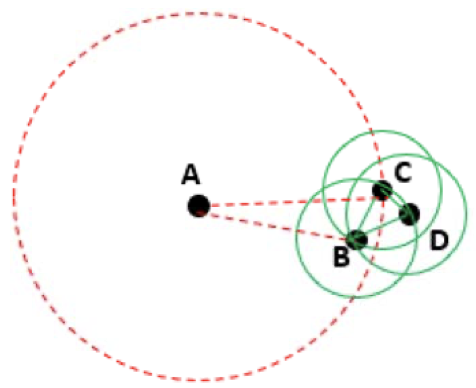
\includegraphics[scale=.75]{chart.png}
\end{center}

\noindent
This question aims at finding the local outlier factor (LOF) for the data points (a) A and (b) C from above figure. Suppose $k$ = 2. We know that: B, C are the two nearest neighbors to A; B and D are the two nearest neighbors to C. We also know the given distances: $d(A, B) = 4$, $d(A, C) = 5$, $d(B, C) = 1.5$, $d(C, D) = 1$, $d(B, D) = 1.2$.

\begin{enumerate}[label=(\alph*)]
    \item LOF (A)
    \item LOF (C)
\end{enumerate}

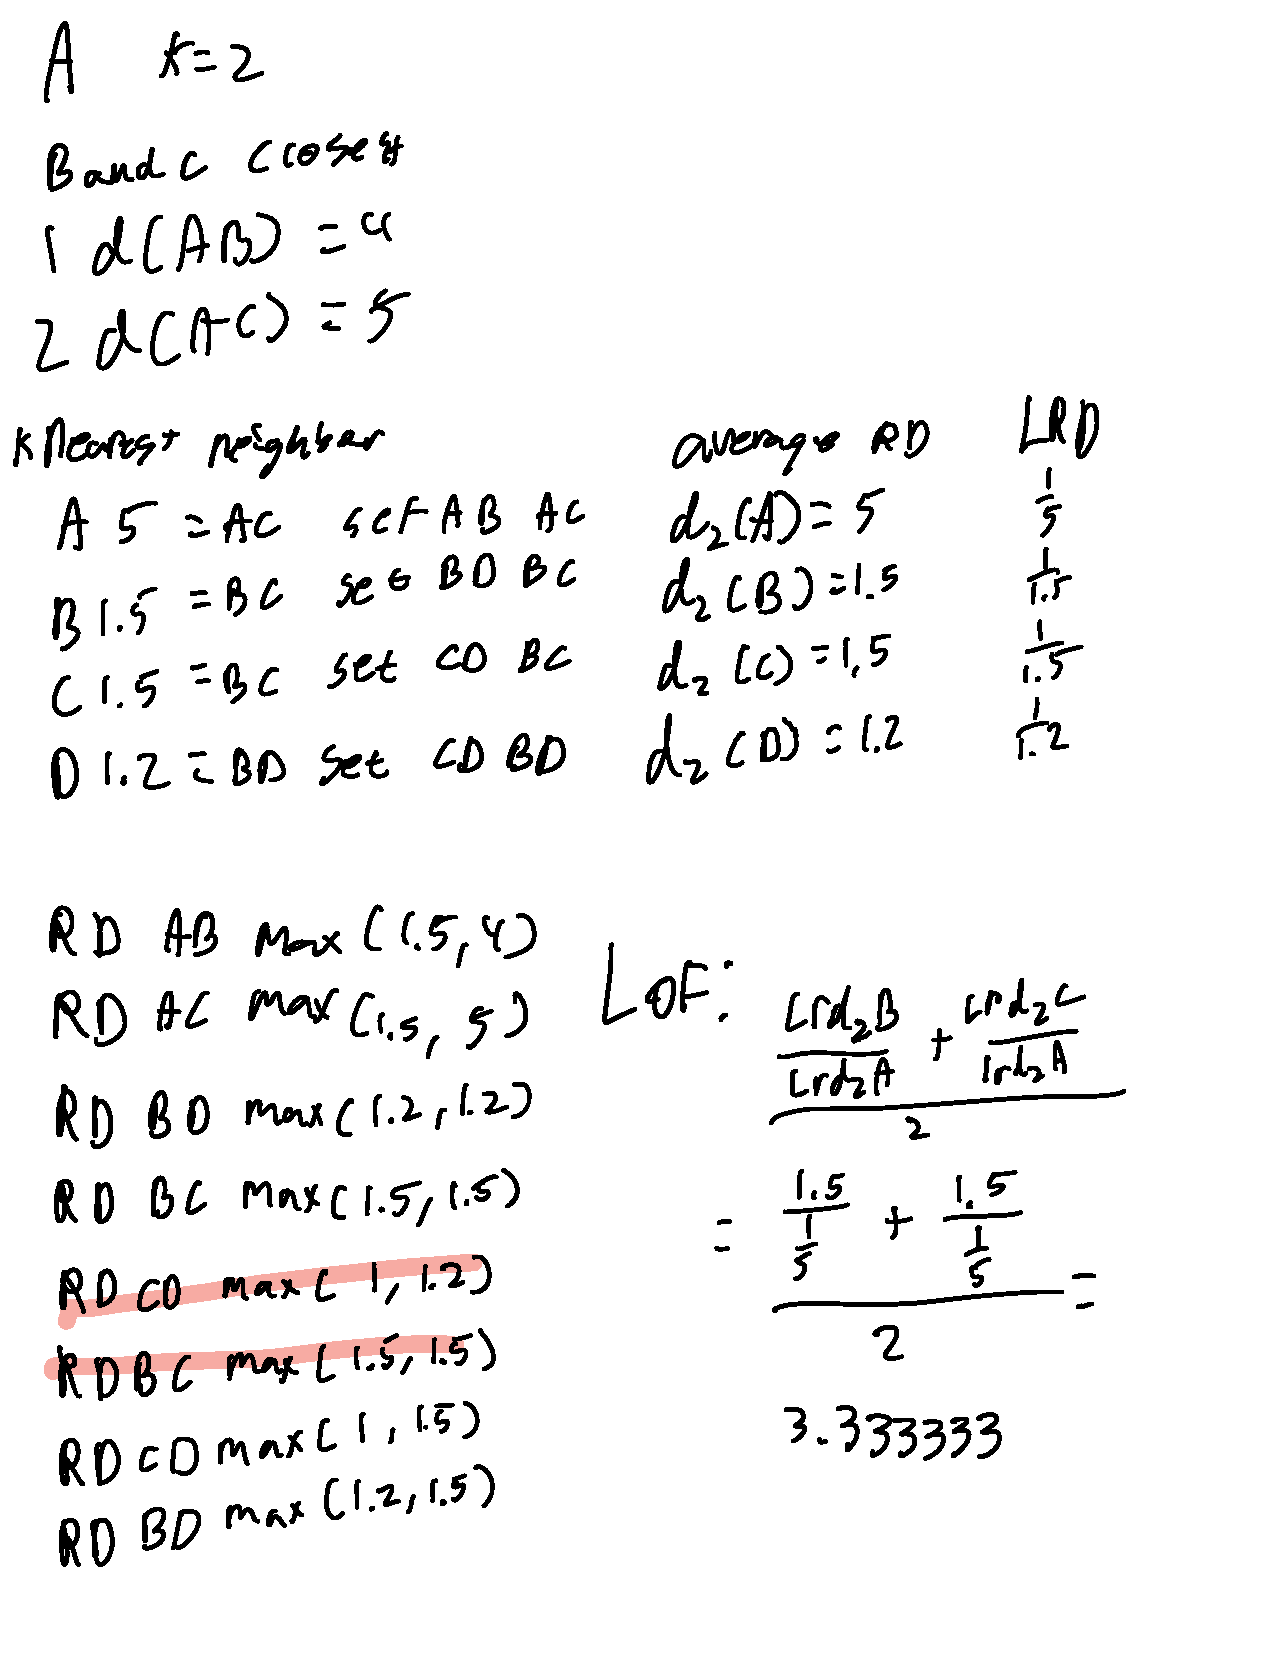
\includepdf[pages=1]{q3.pdf}
\includepdf[pages=2]{q3.pdf}

\end{document}